\documentclass[twocolumn]{jlreq}

\usepackage{ac-room}

\subtitle{筑波大学 産学間連携推進室 成果報告書}% ここは変えない
\title{タイトルをここに書く} % タイトル
\studentnumber{201xxxxxx} % 学籍番号
\author{筑波 太郎} % 名前
\date{} % 日付は空にしておくと出力されない

\begin{document}
%% ここから文書を開始
\twocolumn[
\begin{@twocolumnfalse}
\maketitle
\begin{abstract} % ここに概要を書く
    ここにアブストラクトを書きます。
    ここだけは1段組で表示されるので、ちょっといい感じになります。
    簡潔に研究内容をまとめて、いい感じにしましょう。
    もしまとまりがつかない場合は、構成を考えたほうがいいです。
\end{abstract}
\end{@twocolumnfalse}
]
\section{普通の文章}

こんな感じに美しく組版されます。

\subsection{日本語では}

あのイーハトーヴォのすきとおった風、夏でも底に冷たさをもつ青いそら、うつくしい森で飾られたモリーオ市、郊外のぎらぎらひかる草の波。
またそのなかでいっしょになったたくさんのひとたち、ファゼーロとロザーロ、羊飼のミーロや、顔の赤いこどもたち、地主のテーモ、
山猫博士のボーガント・デストゥパーゴなど、いまこの暗い巨きな石の建物のなかで考えていると、みんなむかし風のなつかしい青い幻燈のように思われます。
では、わたくしはいつかの小さなみだしをつけながら、しずかにあの年のイーハトーヴォの五月から十月までを書きつけましょう\footnote{これはダミーテキストです。注釈は読点の前に入れると良いでしょう}。

\subsection{ラテン語では}

\lipsum[1]\footnote{これもダミーテキストです。出典はキケロらしいですが、ラテン語の文法はめちゃくちゃらしいです}

\section{ソースコードを載せたい}

\subsection{そのまま貼る}

Hello Worldのソースコードを、ソースコード\ref{hello}に示す。

\begin{lstlisting}[language=c,caption=Hello World,label=hello]
#include <stdio.h>

int main()
{
    printf("Hello world!");
}
\end{lstlisting}

\subsection{ファイルから貼る}
ファイルから読み込むやり方はソースコード\ref{file}のようにやります。

\lstinputlisting[language=go,caption=ファイルからコード読み込み,label=file]{./code/binary-tree.go}

\section{画像を載せたい}

画像を載せるときは以下の図\ref{illustya}のようにやります。

\subsection{横幅指定は}

\lstinline{width=\linewidth} にすると横幅がいい感じになります。

\begin{figure}
    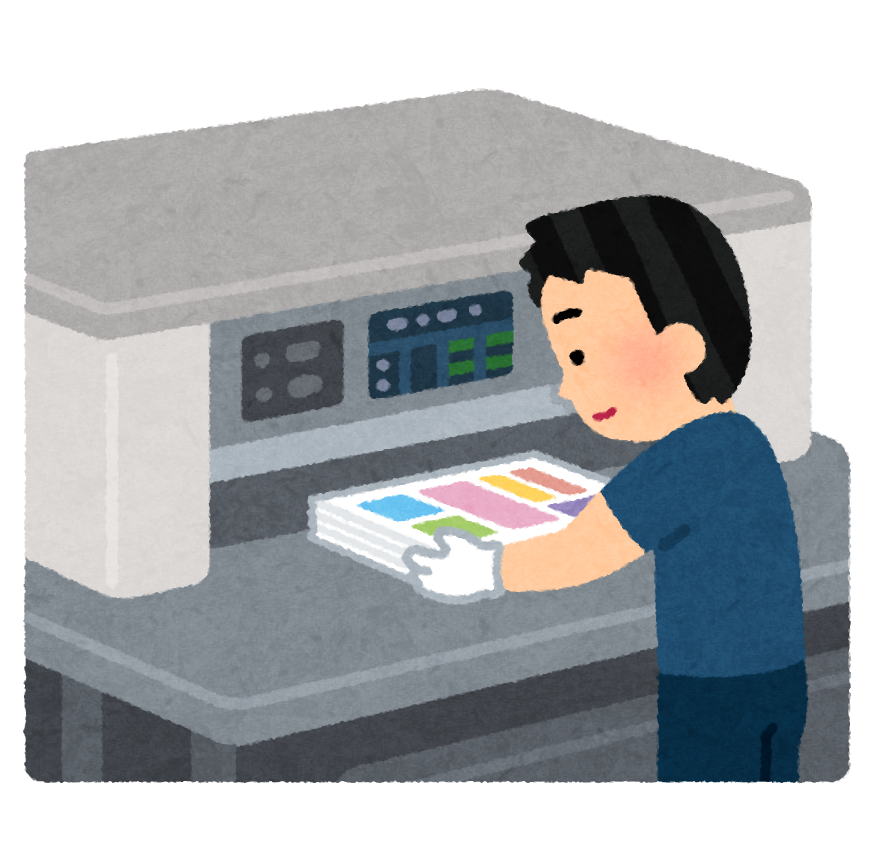
\includegraphics[width=\linewidth]{./img/print_seihon_operator_saidan.png}
    \caption{いらすとやなので安心}
    \label{illustya}
\end{figure}

% 参考文献はmain.bibに書くとここに出力されます
% 参考文献の追加方法はmain.bibを見てくれい
\printbibliography[title=参考文献]

\end{document}

